\section{Complete Results}
\label{sec:complete_results}


\subsection{Complete Accuracy and Cost Tables}
\label{sec:complete_tables}

\begin{table*}[htbp]
\centering
\tiny
\caption{
\textbf{Complete Comparison Table (VQA-v2, GQA, FloodNet, TextVQA).}
Accuracy (\%) and average normalized acquisition cost for each method across datasets and models.
Full-resolution cost $c(\texttt{full})=100$; all other costs are normalized relative to this value.
\textsc{VOILA}-CDF uses a CDF-based threshold in place of the VOI criterion.
\textbf{\textsc{VOILA}} rows are bolded.
}
\label{tab:complete_results_vqa_gqa_flood_textvqa}\label{tab:complete_results}
\resizebox{\linewidth}{!}{
\begin{tabular}{llcccccccc}
\toprule
\multirow{2}{*}{\textbf{Model}} & \multirow{2}{*}{\textbf{Method}}
& \multicolumn{2}{c}{\textbf{VQA-v2}}
& \multicolumn{2}{c}{\textbf{GQA}}
& \multicolumn{2}{c}{\textbf{FloodNet}}
& \multicolumn{2}{c}{\textbf{TextVQA}} \\
\cmidrule(lr){3-4}\cmidrule(lr){5-6}\cmidrule(lr){7-8}\cmidrule(lr){9-10}
& & \textbf{Acc} & \textbf{Cost}
& \textbf{Acc} & \textbf{Cost}
& \textbf{Acc} & \textbf{Cost}
& \textbf{Acc} & \textbf{Cost} \\
\midrule

\multirow{9}{*}{Pixtral-12B-2409}
& Caption              & 49.5 & 7.6   & 42.1 & 7.6   & 21.3 & 7.6   & 78.0 & 7.6   \\
& Resize $32{\times}32$& 33.3 & 15.1  & 37.7 & 15.1  & 25.8 & 15.1  & 18.7 & 15.1  \\
& JPEG Q1              & 57.1 & 37.8  & 59.8 & 37.8  & 30.6 & 37.8  & 25.2 & 37.8  \\
& JPEG Q10             & 70.6 & 53.2  & 68.2 & 53.2  & 45.0 & 53.2  & 46.1 & 53.2  \\
& Full                 & 74.2 & 100.0 & 71.1 & 100.0 & 39.0 & 100.0 & 57.1 & 100.0 \\
& Log-prob Cascade     & 54.0 & 51.9  & 54.9 & 57.7  & 45.2 & 72.3  & 58.4 & 46.3  \\
& \textsc{VOILA}-CDF   & 53.0 & 21.7  & 54.2 & 18.9  & 39.7 & 35.9  & 64.6 & 28.0  \\
& Oracle               & 87.3 & 30.5  & 84.8 & 32.3  & 77.1 & 47.8  & 91.3 & 21.1  \\
& \textbf{\textsc{VOILA}} & \textbf{64.1} & \textbf{38.8} & \textbf{60.5} & \textbf{31.1} & \textbf{45.2} & \textbf{20.7} & \textbf{77.8} & \textbf{8.2} \\
\midrule

\multirow{9}{*}{Llama-4-Maverick (17Bx12E)}
& Caption              & 45.6 & 7.6   & 34.6 & 7.6   & 42.1 & 7.6   & 75.9 & 7.6   \\
& Resize $32{\times}32$& 39.7 & 15.1  & 43.2 & 15.1  & 29.9 & 15.1  & 18.9 & 15.1  \\
& JPEG Q1              & 51.2 & 37.8  & 50.7 & 37.8  & 54.4 & 37.8  & 67.7 & 37.8  \\
& JPEG Q10             & 66.3 & 53.2  & 60.8 & 53.2  & 62.8 & 53.2  & 89.3 & 53.2  \\
& Full                 & 68.4 & 100.0 & 62.9 & 100.0 & 59.7 & 100.0 & 93.7 & 100.0 \\
& Log-prob Cascade     & 45.6 & 7.9   & 34.7 & 7.7   & 41.5 & 11.8  & 75.5 & 10.6  \\
& \textsc{VOILA}-CDF   & 50.3 & 16.9  & 48.8 & 20.4  & 58.8 & 41.9  & 71.7 & 22.3  \\
& Oracle               & 82.4 & 34.3  & 77.9 & 38.7  & 84.0 & 34.9  & 98.1 & 17.7  \\
& \textbf{\textsc{VOILA}} & \textbf{59.7} & \textbf{37.1} & \textbf{53.4} & \textbf{29.5} & \textbf{61.9} & \textbf{19.1} & \textbf{86.4} & \textbf{35.6} \\
\midrule

\multirow{9}{*}{Qwen2-VL-72B-Instruct}
& Caption              & 40.2 & 7.6   & 30.8 & 7.6   & 30.7 & 7.6   & 73.3 & 7.6   \\
& Resize $32{\times}32$& 44.7 & 15.1  & 47.9 & 15.1  & 73.8 & 15.1  & 22.2 & 15.1  \\
& JPEG Q1              & 60.6 & 37.8  & 61.6 & 37.8  & 23.5 & 37.8  & 66.0 & 37.8  \\
& JPEG Q10             & 74.7 & 53.2  & 71.2 & 53.2  & 39.8 & 53.2  & 92.1 & 53.2  \\
& Full                 & 77.6 & 100.0 & 73.5 & 100.0 & 58.6 & 100.0 & 97.1 & 100.0 \\
& Log-prob Cascade     & 40.2 & 7.7   & 30.8 & 7.6   & 70.2 & 59.9  & 73.3 & 7.6   \\
& \textsc{VOILA}-CDF   & 50.5 & 16.3  & 53.6 & 23.0  & 61.5 & 52.6  & 73.3 & 26.3  \\
& Oracle               & 87.3 & 30.9  & 84.7 & 33.7  & 86.3 & 29.4  & 99.2 & 17.5  \\
& \textbf{\textsc{VOILA}} & \textbf{64.4} & \textbf{37.3} & \textbf{60.0} & \textbf{28.9} & \textbf{73.4} & \textbf{13.0} & \textbf{86.9} & \textbf{33.1} \\
\midrule

\multirow{9}{*}{LLaVA-1.5-7B-hf}
& Caption              & 57.7 & 7.6   & 63.2 & 7.6   & 67.0 & 7.6   & 79.0 & 7.6   \\
& Resize $32{\times}32$& 59.5 & 15.1  & 66.4 & 15.1  & 66.7 & 15.1  & 26.0 & 15.1  \\
& JPEG Q1              & 58.3 & 37.8  & 62.9 & 37.8  & 48.7 & 37.8  & 57.9 & 37.8  \\
& JPEG Q10             & 70.7 & 53.2  & 72.2 & 53.2  & 69.4 & 53.2  & 72.7 & 53.2  \\
& Full                 & 73.1 & 100.0 & 74.1 & 100.0 & 67.3 & 100.0 & 75.7 & 100.0 \\
& Log-prob Cascade     & 62.7 & 35.6  & 69.3 & 36.5  & 66.9 & 12.4  & 75.9 & 42.9  \\
& \textsc{VOILA}-CDF   & 62.9 & 14.6  & 68.0 & 19.0  & 68.9 & 22.9  & 69.3 & 22.5  \\
& Oracle               & 86.6 & 26.1  & 87.3 & 24.3  & 77.5 & 30.9  & 92.7 & 18.9  \\
& \textbf{\textsc{VOILA}} & \textbf{66.5} & \textbf{26.2} & \textbf{69.5} & \textbf{25.9} & \textbf{68.6} & \textbf{15.2} & \textbf{79.2} & \textbf{9.4} \\
\midrule

\multirow{9}{*}{Qwen2.5-VL-7B-Instruct}
& Caption              & 35.9 & 7.6   & 39.7 & 7.6   & 35.3 & 7.6   & 71.8 & 7.6   \\
& Resize $32{\times}32$& 48.7 & 15.1  & 45.9 & 15.1  & 50.1 & 15.1  & 23.8 & 15.1  \\
& JPEG Q1              & 57.0 & 37.8  & 47.4 & 37.8  & 55.5 & 37.8  & 64.6 & 37.8  \\
& JPEG Q10             & 72.6 & 53.2  & 59.0 & 53.2  & 63.5 & 53.2  & 92.2 & 53.2  \\
& Full                 & 77.8 & 100.0 & 66.2 & 100.0 & 62.1 & 100.0 & 97.7 & 100.0 \\
& Log-prob Cascade     & 61.4 & 74.7  & 52.0 & 74.8  & 53.2 & 51.2  & 71.1 & 64.1  \\
& \textsc{VOILA}-CDF   & 53.0 & 21.1  & 53.1 & 24.2  & 50.4 & 35.6  & 75.2 & 26.6  \\
& Oracle               & 88.0 & 31.7  & 82.5 & 36.2  & 78.5 & 39.4  & 99.3 & 18.0  \\
& \textbf{\textsc{VOILA}} & \textbf{63.1} & \textbf{34.1} & \textbf{55.0} & \textbf{27.8} & \textbf{56.6} & \textbf{22.8} & \textbf{88.2} & \textbf{38.0} \\
\midrule

\multirow{9}{*}{Qwen3-VL-235B-A22B-Instruct}
& Caption              & 57.7 & 7.6   & 29.0 & 7.6   & 54.6 & 7.6   & 75.9 & 7.6   \\
& Resize $32{\times}32$& 50.4 & 15.1  & 53.3 & 15.1  & 31.3 & 15.1  & 23.9 & 15.1  \\
& JPEG Q1              & 63.7 & 37.8  & 62.3 & 37.8  & 67.5 & 37.8  & 72.2 & 37.8  \\
& JPEG Q10             & 76.9 & 53.2  & 70.3 & 53.2  & 77.5 & 53.2  & 95.1 & 53.2  \\
& Full                 & 79.1 & 100.0 & 73.2 & 100.0 & 74.1 & 100.0 & 98.5 & 100.0 \\
& Log-prob Cascade     & 62.8 & 41.8  & 65.0 & 83.8  & 57.8 & 20.9  & 77.2 & 64.4  \\
& \textsc{VOILA}-CDF   & 63.3 & 17.7  & 55.4 & 21.2  & 70.1 & 62.1  & 78.2 & 24.9  \\
& Oracle               & 89.7 & 25.5  & 83.8 & 34.0  & 85.4 & 31.3  & 99.7 & 15.9  \\
& \textbf{\textsc{VOILA}} & \textbf{71.5} & \textbf{37.4} & \textbf{59.0} & \textbf{24.4} & \textbf{75.1} & \textbf{25.1} & \textbf{90.4} & \textbf{35.0} \\
\bottomrule
\end{tabular}
}
\end{table*}


\subsection{Fidelity Selection Distributions}
\label{sec:fidelity_distributions}

\begin{figure*}[t]
    \centering
    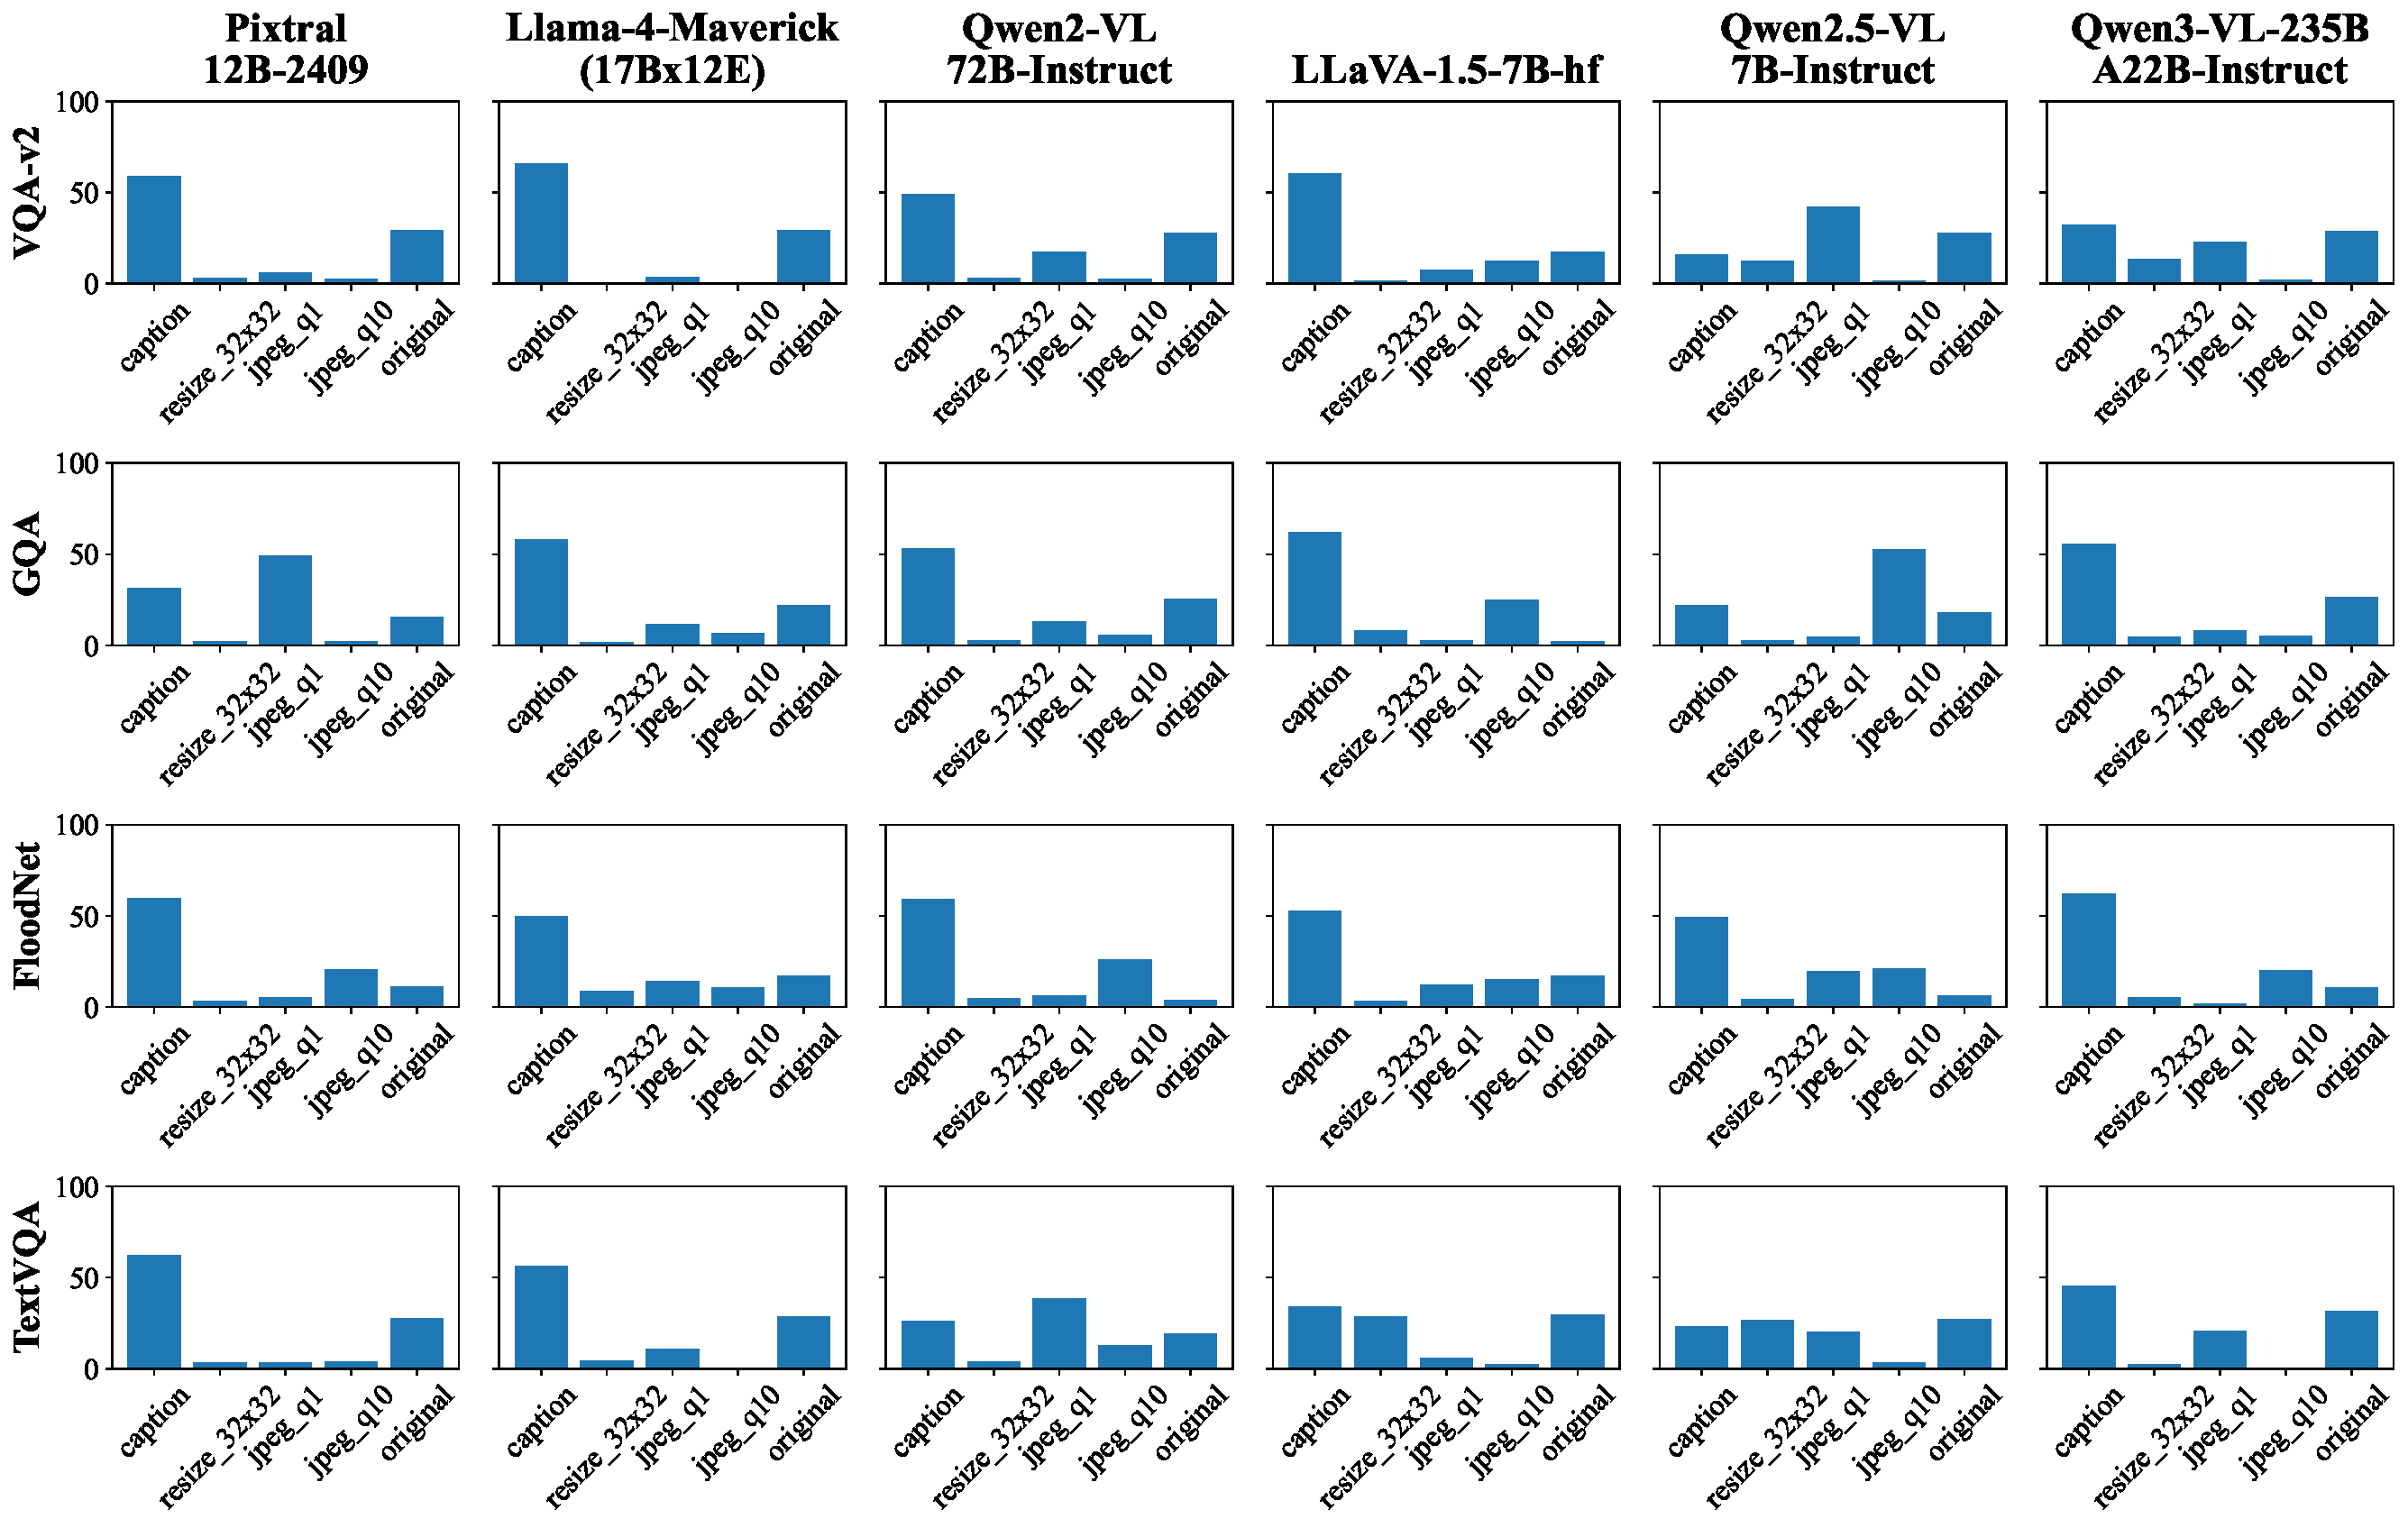
\includegraphics[width=\linewidth]{plots/fidelity_distribution_plot.pdf}
    \caption{
    \textbf{Learned fidelity selection distributions under \textsc{VOILA} routing.}
    Each subplot reports the percentage of queries routed to each input fidelity by \textsc{VOILA}, across four datasets (rows) and six vision--language models (columns).
    Low-cost representations (captions and low-resolution thumbnails) dominate across all settings, while higher-cost fidelities (JPEG Q1/Q10 and full-resolution images) are selected selectively when expected utility justifies their acquisition cost.
    }
    \label{fig:voila_fidelity_distribution}
\end{figure*}


\subsection{LoCoMo Memory Recall Results}

\begin{table}[htb]
\centering
\small
\setlength{\tabcolsep}{4pt}
\caption{\textbf{LoCoMo memory recall (Acc\% / Cost).}
\textsc{VOILA} trained on VQA-v2+GQA, evaluated on LoCoMo (OOD). Limited to two VLMs due to GPT-4o answer-generation cost.
}
\label{tab:locomo_ultracompact_appendix}
\resizebox{\columnwidth}{!}{
\begin{tabular}{lccccc}
\toprule
\textbf{Model} & \textbf{Caption} & \textbf{Full} & \textbf{BERT Router} & \textbf{LLM Router} & \textbf{\textsc{VOILA}} \\
\midrule
Pixtral-12B    & 32.5 / 7.6 & 46.7 / 100 & 42.0 / 43.3 & 38.5 / 43.3 & \textbf{41.1 / 25.4} \\
Qwen2.5-VL-7B  & 26.8 / 7.6 & 73.0 / 100 & 57.5 / 44.5 & 58.5 / 43.3 & \textbf{55.9 / 30.6} \\
\bottomrule
\end{tabular}}
\end{table}

\subsection{Out-of-Distribution Transfer Results}
\label{sec:ood_results}

\begin{table}[htb]
\centering
\small
\setlength{\tabcolsep}{3pt}
\renewcommand{\arraystretch}{0.95}
\caption{\textbf{Out-of-distribution transfer (Acc\% / Cost).}
\textsc{VOILA} trained on one dataset and evaluated on the other, with $\lambda$/$\tau$ fixed to source-domain values (zero-shot OOD). Costs remain well below full-resolution (100) under both transfer directions.}
\label{tab:ood_pixtral_compact_appendix}
\begin{tabular}{lcc}
\toprule
\textbf{Model}
& \textbf{VQA$\rightarrow$GQA}
& \textbf{GQA$\rightarrow$VQA} \\
\midrule
Llama-4-Maverick & 46.5 / 26.0 & 52.8 / 25.5 \\
LLaVA-1.5-7B    & 65.7 / 18.6 & 65.6 / 35.6 \\
Pixtral-12B      & 54.1 / 34.4 & 58.8 / 32.0 \\
Qwen2.5-VL-7B   & 51.2 / 26.7 & 49.8 / 21.7 \\
Qwen2-VL-72B    & 51.9 / 24.4 & 53.4 / 24.5 \\
Qwen3-VL-235B   & 38.3 / 25.2 & 62.2 / 29.7 \\
\bottomrule
\end{tabular}
\end{table}

\pagebreak
